\documentclass[11pt,twocolumn,twoside]{IEEEtran}
\usepackage{amsmath}
\usepackage[pdftex]{epsfig}
\usepackage{amsfonts}
\usepackage{amssymb}
\usepackage{fancyhdr}
\usepackage{url}
\include{graphicsx}

\pagestyle{fancy}
%\renewcommand{\headrulewidth}{0pt}
\renewcommand{\footrulewidth}{0pt}
\rhead{
\includegraphics[height=0.6in]{cilogo.png}}
\fancyhead[LO]{\sc sci-wms\ldots} % shorter form of title to fit in space
\fancyhead[LE]{\sc Mayer, McKenna, Knee} % author list or et al., to fit in space
\chead{}
\cfoot{}

\newcommand{\comt}{COMT}
\newcommand{\ioos}{IOOS}
\newcommand{\sura}{SURA}
\newcommand{\ogc}{OGC}
\newcommand{\wms}{WMS}
\newcommand{\csw}{CSW}
\newcommand{\ugrid}{u-grid}
\newcommand{\cgrid}{c-grid}
\newcommand{\ncml}{NcML}
\newcommand{\noaa}{NOAA}
\newcommand{\ngdc}{NGDC}
\newcommand{\opendap}{OpenDAP}
\newcommand{\netcdf}{NetCDF}
\newcommand{\sciwms}{sci-wms}
\newcommand{\Sciwms}{Sci-wms}
\newcommand{\adcirc}{ADCIRC}
\newcommand{\fvcom}{FVCOM}
\newcommand{\selfe}{SELFE}
\newcommand{\slosh}{SLOSH}
\newcommand{\mdl}{MDL}
\newcommand{\und}{UND}
\newcommand{\usf}{USF}
\newcommand{\vims}{VIMS}
\newcommand{\umass}{UMASS}
\newcommand{\dal}{DAL}
\newcommand{\tamu}{TAMU}


\begin{document}
\title{\vspace{0.2in}\sc sci-wms:Python based Web Mapping Service for Visualizing Geospatial data}

\author{Brandon A. Mayer$^{1,2}$, Brian McKenna$^{2}$, Kelly Knee$^{2}$\thanks{Brown University School Of Engineering$^{1}$, RPS-Applied Science Associates, South Kingston RI$^{2}$, Brandon\_Mayer@brown.edu, BMcKenna@asascience.com, KKnee@asascience.com}}

\maketitle
\thispagestyle{fancy}

\begin{abstract}
\sciwms{} is used as an extensible visualization tool for qualitativly
assessing society-critical oceanagraphic applications including:
forecasts, risk assessment, model comparison and algorithmic/parameter
selection. This abstract outlines the implementation and technology
stack for visualizing geospatial coastal forecasting (CF) data using
sci-wms~\cite{wms14}.\footnote{https://github.com/asascience-open/sci-wms}
Specifically, detailing the use case for deploying \sciwms{} for visualizing
model data and simulations within the scope of the U.S. \ioos{} Coastal
and Ocean Modeling Testbed project.~\cite{luettich13}
\end{abstract}

\section{Motivation}
The U.S. Integrated Ocean Observing System (\ioos{}) Coastal and Ocean
Modeling Testbed (\comt{}) was formed to unify otherwise disparate
entities in government, academia and industry to leverage the
proliferation of coastal data and modeling techniques to combat
natural and man-made stressors by accelerating the turnaround from
research and development to operational application of
society-critical applications including: forecasting, model comparison,
model skill assessment, and algorithmic/parameterization
improvements~\cite{luettich13}. Key to the U.S. \ioos{} \comt{}
mission is an extensible and universally available tool for quickly
visualizing and assessing coastal modeling data.

\section{\sciwms{}}
\Sciwms{} is an implementation of the Open Geospatial Consortium's
(\ogc{}) Web Map Service (\wms{}) standard which specifies a http
interface for generating rasterized visualizations of geospatial
data~\cite{wms14}. Sci-wms is implemented in python using the
Django\footnote{\url{https://www.djangoproject.com/}} web framework
and standard cross-platform numerical software, NumPy and
Matplotlib~\cite{numpy11, hunter07} for generating visual
content. Vital to the efficiency of \sciwms{} is the
abstraction of an oceanagraphic dataset into two entities: a topology,
defined as a geo-referenced spatial structure and model data as
visualized in figure~\ref{fig:sciwms_topology_endpoints}. \Sciwms{}
creates a local topology cache for efficiently computing spatial
neighborhoods with respect to topology structure.  For storage
efficiency, model data is not replicated when hosted externally but
reference via web-enabled endpoints. Because
geospatial \wms{} requests are commonly restricted to a subset of the
earth surface, \sciwms{} uses the local topology to compute the
subset of model data needed to fulfill each request prior to
accessing the external data. Furthermore, by classifying
topologies as either regular or unstructured, efficient algorithms and
data structures are exploited to optimize the computation of relevant
model data subsets.

\begin{figure}
  \centering
  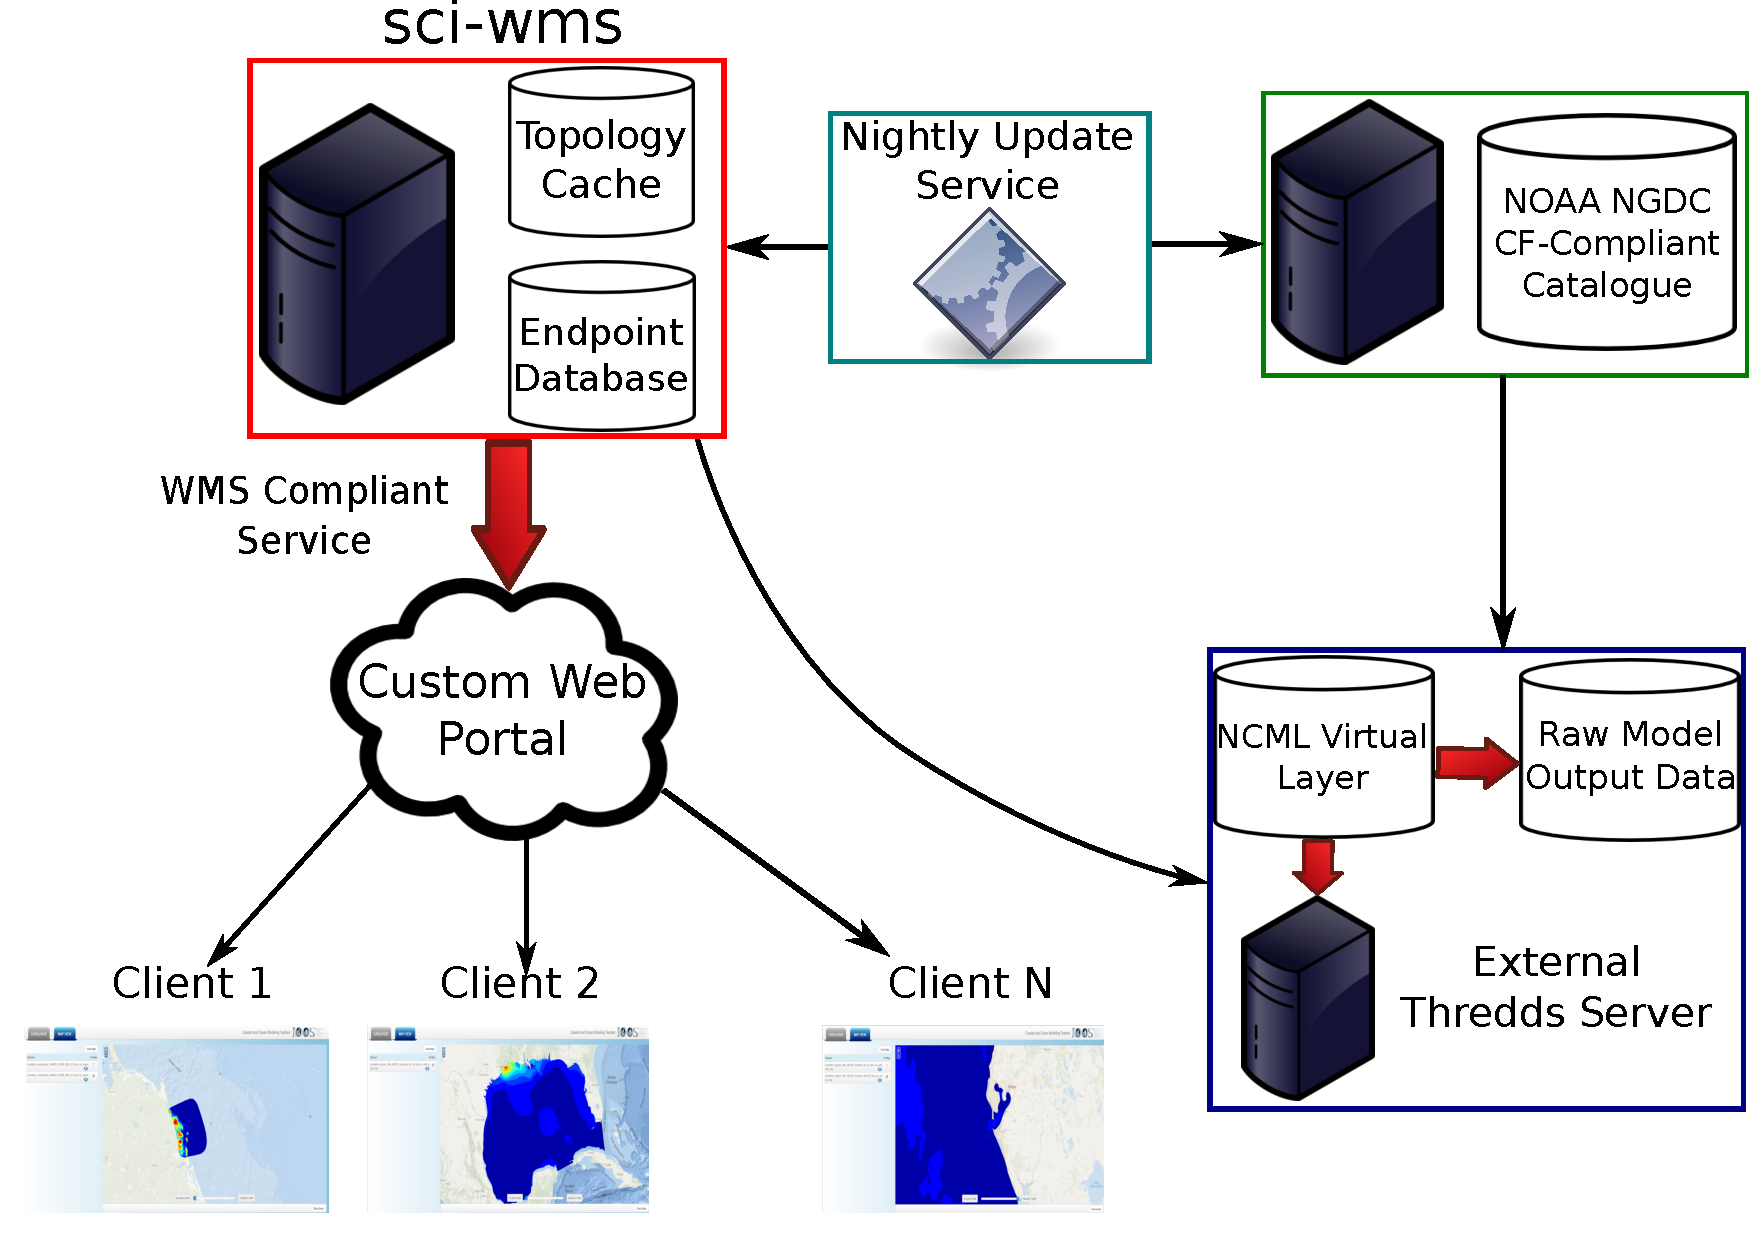
\includegraphics[width=\columnwidth]{./figs/overview.pdf}
  \caption{Overview of the \sciwms{} deployment for the U.S. \ioos{}
    \comt{} project. \Sciwms{} updates its topology and endpoint
    database via a nightly service which queries CF-Compliant datasets
    cataloged by \ngdc{}. Model data is hosted on an external web
    server through an \ncml{} facade accessible to \sciwms{} through
    \opendap{} as a single \netcdf data structure. \Sciwms then
    responds to http requests made simultaneously by multiple clients
    interfacing through a custom built web-portal.}
  \label{fig:overview1}
\end{figure}

\begin{figure}
  \centering
  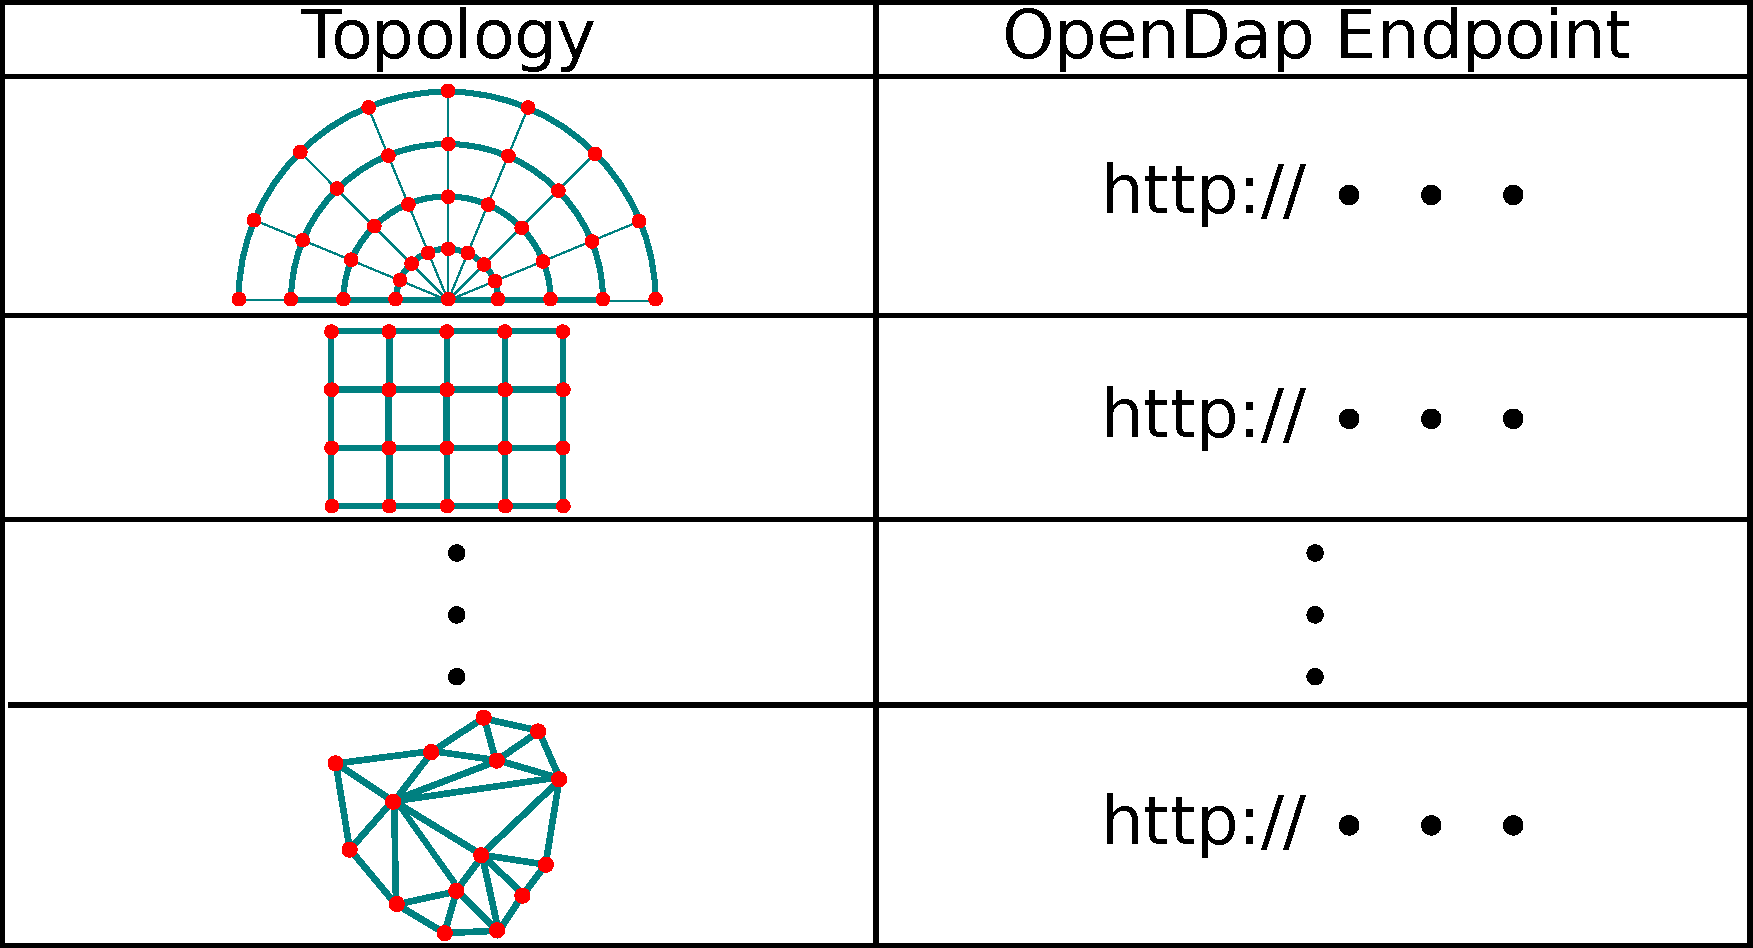
\includegraphics[width=\columnwidth]{./figs/sciwms_db_topology_endpoints.pdf}
  \caption{\Sciwms{} topology and endpoint data store. Typologies are
    classified as \ugrid{} or \cgrid{} for efficient geospatial
    queries and remote model data access.}
  \label{fig:sciwms_topology_endpoints}
\end{figure}

\section{Deploying \sciwms{} for the U.S. \ioos{} \comt{} Testbed}
While \sciwms{} is a general software solution for geospatial
visualization, it is a key component in realizing the U.S. \ioos{}
\comt{} mission, facilitating qualitative model comparisons and
aggregation through a unified visualization
framework. Figure~\ref{fig:overview1} outlines the cyberinfrastructre
behind the deployment of \sciwms{} for the \comt{} project.

Raw coastal data is hosted by the Southeastern Universities Research
Association (\sura{}) on a dedicated server for the \comt{}
project~\cite{luettich12}. Each data set may consist of multiple files
in different formats, and may be the result of very different models
run by various institutions with disparate computing
resources. However, accompanying each dataset is an \ncml{} virtual
layer which exposes each dataset as a single \netcdf{} object which
may be accessed via \opendap{}. Furthermore, the \ncml facade presents
a consistent set of meta information in accordance to
CF-Conventions~\cite{cf} so services like \sciwms{} can access
the data through a uniform interface.

Once an \ncml{} file is confirmed to be CF-Compliant, the dataset is
indexed by \noaa{}\footnote{National Oceanic and Atmospheric
  Administration}--\ngdc{}\footnote{National Geophysical Data Center}
and made accessible via an \ogc{} catalogue web service (\csw{}). A executable
queries the \ngdc{} catalogue at regular intervals for new or modified
datasets and automatically updates both the topologies and \opendap{}
links in the \sciwms{} database. At any time \sciwms{} is able to
respond to queries for visualizations of any registered dataset by
multiple users simultaneously.

\Sciwms{} is capable of visualizing data
associated with the first phase of \comt{} coastal and ocean
prediction: {\em estuarine hypoxia, shelf hypoxia and coastal
  inundation}~\cite{luettich13}. For each coastal modeling challenge,
\sciwms{} is successfully generating visualizations resulting from
\adcirc{}, \fvcom{}, \selfe{} and \slosh{} models run by scientists at
\mdl{}, \und{}, \usf{}, \vims{}, \umass{}, \dal{}, \tamu{} and
\noaa{}. The \ioos{} \comt{} use case is an example of how \sciwms{}
can be leveraged as an effective tool for delivering consistent
visualizations of scientific data to a diverse community utilizing
various sophisticated modeling technologies.


\bibliographystyle{ieeetr}
\bibliography{ci_mayer}
%% \bibliography{bibfile,benherzog}

\end{document}
